
\noindent{\Large \bf Supplementary Material}

\bigskip

\section{Data collection}
1- Data collection: key words, clade (ordinal) metacharacters, Google Search terms, Google Search protocol, Google Search rarefaction curve.

\subsection{search terms}
The searched mammalian order terms are available in $search_terms_latin.txt$ or $search_terms_meta.txt$. The file containing the meta names is the Latin name files but with replacing the latin suffixes ([ia|ata|ea|a]) by a joker character (*) and by replacing the first letter by a upper/lower case meta character (e.g. [Aa]).
Mammalia; Monotremata; Marsupialia; Placentalia; Macroscelidea; Afrosoricida; Tubulidentata; Hyracoidea; Proboscidea; Sirenia; Pilosa; Cingulata; Scandentia; Dermoptera; Primates; Lagomorpha; Rodentia; Erinaceomorpha; Soricomorpha; Cetacea; Artiodactyla; Cetartiodactyla; Chiroptera; Perissodactyla; Pholidota; Carnivora; Didelphimorphia; Paucituberculata; Microbiotheria; Dasyuromorphia; Peramelemorphia; Notoryctemorphia and Diprotodontia.

\subsubsection{Ross Mounce data set}
I selected all the matrices containing at least one of the mammalian orders names from Ross Mounce GitHub $cladistic-data/nexus_files$ repository (accessed on the 02/12/2014).

\subsubsection{Graeme Lloyd}
Selecting the downloadable matrices

\subsubsection{Morphobank}
\textit{order}

\subsubsection{Google scholars}
20 first results since 2010 with the following exact key words:

\texttt{\textit{order} ("morphology" OR "morphological" OR "cladistic") AND characters matrix paleontology phylogeny}

We selected only the 20 first results per search term because only the 50 first of the 660 papers added 425 living OTUs.

\begin{figure}[!htbp]
\centering
    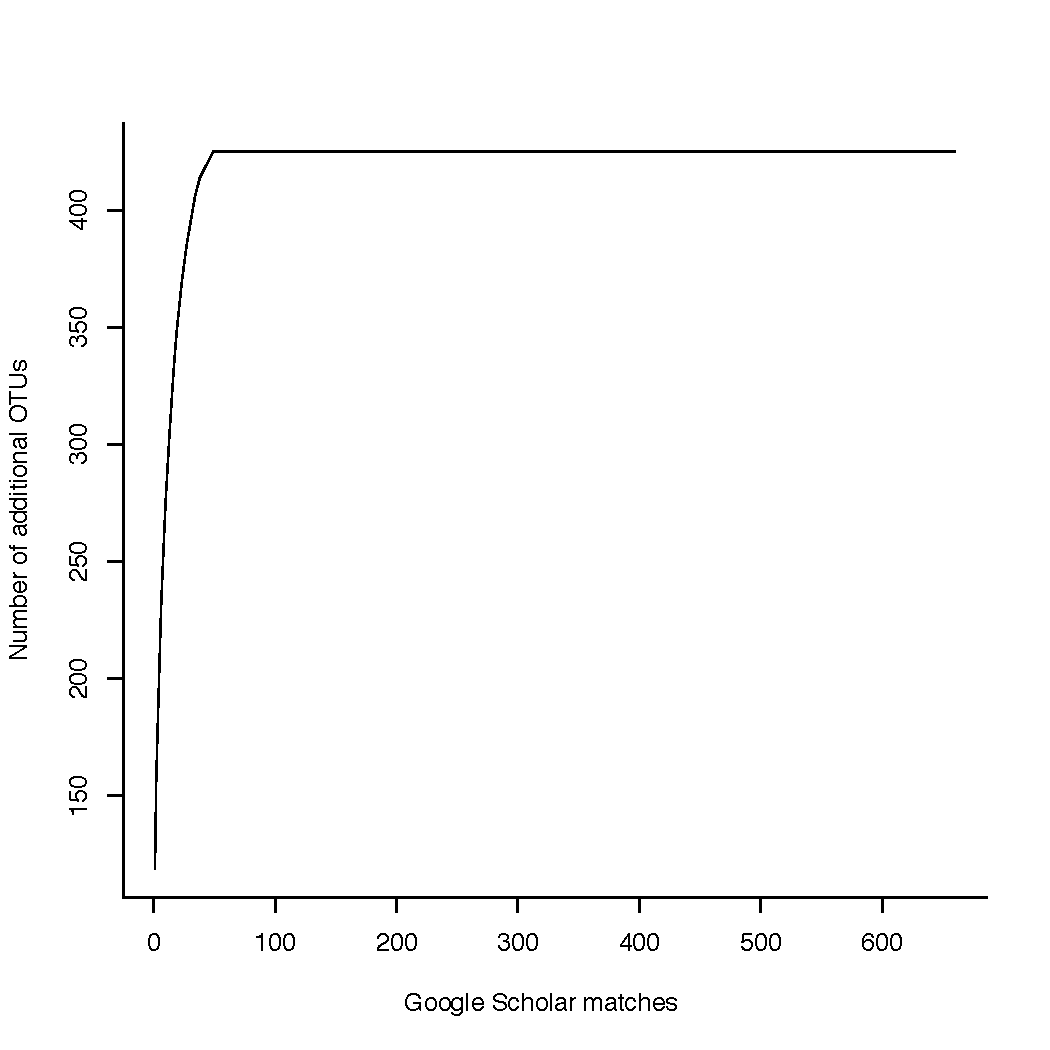
\includegraphics[width=1\textwidth]{Supplementary/Supp_figure_google_searches.pdf}
\caption{Google searches additional OTUs rarefaction curve. The x axis represent the number of google scholar matches (papers, books or abstracts) and the y axis represents the cumulative number of additional living OTUs per google scholar match.}
\label{Supp_figure_google_searches}
\end{figure}


\subsection{Wrong Bionmial names and typos}
I fixed the wrong bionomial names format (e.g. H. sapiens) into the correct ones (e.g. Homo sapiens) manually using the abreviation list in the concerned publications. We then applied our taxonomic matching algorithm to classify the OTUs as either living or fossil.

\begin{figure}[!htbp]
\centering
    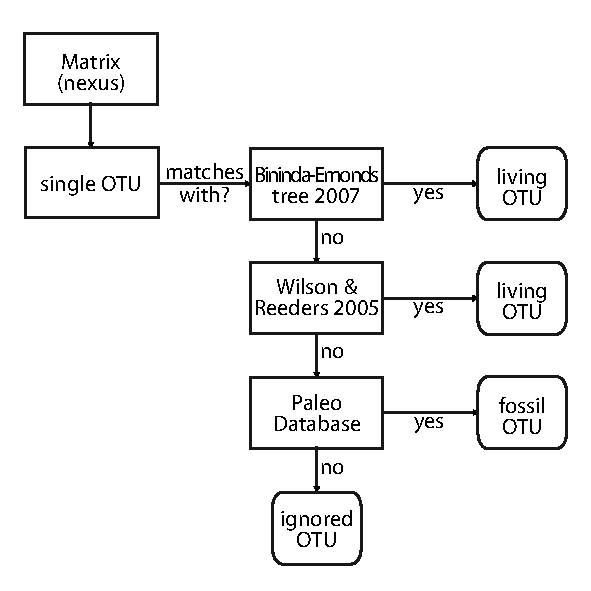
\includegraphics[width=1\textwidth]{Supplementary/Supp_figure_Taxonomic_algorithm.pdf}
\caption{Taxonomic matching algorithm used in this study. For each matrix, each operational taxonomic units (OTU) is matched with the super tree from Fritz 2009. If the OTU matches, then it is classified as living. Else it is matched with the Wilson \& Reeders 2005 taxonomy list. If the OTU matches, then it is classified as living. Else it is matched with the Paleo Database list of mammals. If the OTU matches, then it is classified as fossil. Else it is ignored.}
\label{Supp_figure_Taxonomic_algorithm}
\end{figure}

\bibliographystyle{vancouver}
\bibliography{Supp_References}


\section{Data structure}
%Tables
%Figures

\section{Supplementary results}
